\documentclass{article}
\usepackage{listings}
\usepackage{xcolor}
\lstset { %
    language=C++,
    backgroundcolor=\color{black!5}, % set backgroundcolor
    basicstyle=\footnotesize,% basic font setting
    breaklines
}
\usepackage{graphicx}
\usepackage{url}
\usepackage{hyperref}
\hypersetup{
    colorlinks=true,
    linkcolor=blue,
    filecolor=magenta,      
    urlcolor=cyan,
}


\title{Development of the Planes Game}
\date{2017-06-09}
\author{Cristian Cucu}
\begin{document}
\maketitle
\newpage
\lstset{language=C++}
\section{Introduction}

\subsection{Game Description}
The game is a variant of the classical \href{https://en.wikipedia.org/wiki/Battleship_(game)}{battleship game}. The ships will be here called planes and are shown in \ref{fig:board}.
\begin{figure}[h]
  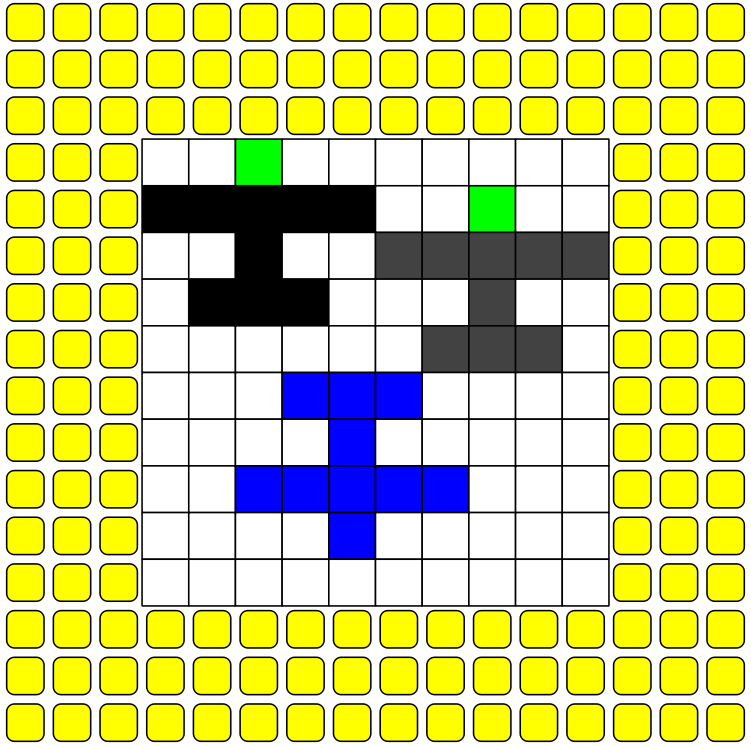
\includegraphics[width = \textwidth]{BoardWithPlanes.png}
  \caption{Board game with 3 planes}
  \label{fig:board}
\end{figure}

\subsection{Requirements Analysis}
We need an object that describes a plane object which should at least contain information about the position of the plane on the game grid, the orientation of the plane, the shape of a plane. Additionaly we would need a game board/grid object. It should not be restricted to a specific geometry, should know where each plane is positioned and how many planes there are. Since the game is played against the computer there should be a kind of strategy object that decides the computer's next move.
A graphical interface for editing the board and playing the game is also required together with the associated controller objects.


\section{The Plane Object}
A plane object is defined through the position of its head  (plane front) and its orientation (see \ref{fig:plane_orientations}).  We assume that each plane exists somewhere in its own reference system and in its own rectangular grid - that is a plane object is not explicitly related to a game board object. 

\begin{figure}[h]
  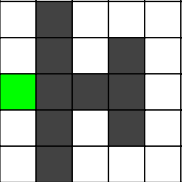
\includegraphics[width = 3cm]{PlaneEastWest.png}
  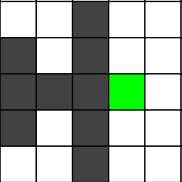
\includegraphics[width = 3cm]{PlaneWestEast.png}
  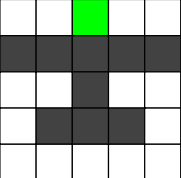
\includegraphics[width = 3cm]{PlaneNorthSouth.png}
  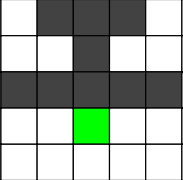
\includegraphics[width = 3cm]{PlaneSouthNorth.png}
  \caption{Possible plane orientations}
  \label{fig:plane_orientations}
\end{figure}

\subsection{Class declaration}
\begin{lstlisting}[caption = {Plane class declaration}, captionpos = b, label=plane_declaration]
class Plane
{
public:
    enum Orientation {NorthSouth = 0, SouthNorth = 1, WestEast = 2, EastWest = 3};

private:
    //plane orientation
    Orientation m_orient;
    //coordinates of the position of the head of the plane
    int m_row, m_col;

public:
    //Various constructors
    Plane();
    Plane(int row, int col, Orientation orient);
    Plane(const QPoint& qp, Orientation orient);

    //setter and getters
    //gives the planes orientation
    Orientation orientation() const {return m_orient; }
    //gives the plane head's row and column
    int row() const { return m_row; }
    int col() const { return m_col;}
    //sets the plane head position
    void row(int row) { m_row = row; }
    void col(int col) { m_col = col; }
    void orientation(Orientation orient) { m_orient = orient; }
    //gives the coordinates of the plane head
    QPoint head() const { return QPoint(m_row, m_col); }

    //operators
    //compares two planes
    bool operator==(const Plane& pl1) const;
    //equals operator
    void operator=(const Plane& pl1);
    //translates a plane by a QPoint
    Plane operator+(const QPoint& qp);

    //geometrical transformations
    //clockwise rotation of planes
    void rotate();
    //translation with given offset in a grid with row and col rows and columns
    //if the future head position is not valid do not translate
    void translateWhenHeadPosValid(int offsetX, int offsetY, int row, int col);

    //other utility functions
    //tests whether a QPoint is a planes head
    bool isHead(const QPoint& qp) const { return qp == head(); }
    //checks if a certain point on the grid is on the plane
    bool containsPoint(const QPoint& qp) const;
    //returns whether a plane position is valid (the plane is completely contained inside the grid) in a grid with row and col
    bool isPositionValid(int row, int col) const;
    //generates a random number from 0 and valmax-1
    static int generateRandomNumber(int valmax);
    //displays the plane
    QString toString() const;
};
\end{lstlisting}

In the above class definition appear types that are not pure C++ types, but are defined in the Qt library. They restrict the use of the Plane class to a Qt program. One is the QPoint type, which defines a 2D coordinate. The second is the QString which represents a string, the analog of std::string in the Qt library. 

\subsection {Method Implementation}
\begin{lstlisting}[caption = {Plane class methods}, captionpos = b, label=plane_implementation]
//Various constructors
Plane::Plane() {
    m_row = 0;
    m_col = 0;
    m_orient = NorthSouth;
}

Plane::Plane(int row, int col, Orientation orient) {
    m_row = row;
    m_col = col;
    m_orient = orient;
}

Plane::Plane(const QPoint &qp, Orientation orient) {
    m_row = qp.x();
    m_col = qp.y();
    m_orient = orient;
}

//equality operator
bool Plane::operator==(const Plane &pl1) const {
    return ((pl1.m_row == m_row) && (pl1.m_col == m_col) && (pl1.m_orient == m_orient));
}

//assignment operator
void Plane::operator=(const Plane &pl1) {
    m_row = pl1.m_row;
    m_col = pl1.m_col;
    m_orient = pl1.m_orient;
}

//Clockwise 90 degrees rotation of the plane
void Plane::rotate() {
    switch(m_orient)
    {
    case NorthSouth:
        m_orient = EastWest;
        break;
    case EastWest:
        m_orient = SouthNorth;
        break;
    case SouthNorth:
        m_orient = WestEast;
        break;
    case WestEast:
        m_orient = NorthSouth;
        break;
    default:
        return;
    }
}

//checks to see if a plane contains a certain point
//uses a PlanePointIterator which enumerates
//all the points on the plane
bool Plane::containsPoint(const QPoint &qp) const {
    PlanePointIterator ppi(*this);

    while(ppi.hasNext())
    {
        QPoint qp1=ppi.next();
        if(qp==qp1)
            return true;
    }

    return false;
}

//Checks to see if the plane is
//in its totality inside a grid
//of size row X col
bool Plane::isPositionValid(int row, int col) const {
    PlanePointIterator ppi(*this);

    while(ppi.hasNext())
    {
        QPoint qp = ppi.next();
        if(qp.x()<0 || qp.x()>=row)
            return false;
        if(qp.y()<0 || qp.y()>=col)
            return false;
    }

    return true;
}

//utility function
//generates a random number
int Plane::generateRandomNumber(int valmax) {
    double rnd = rand()/ static_cast<double>(RAND_MAX);
    if (rnd==1.0)
        rnd = 0.5;
    int val = static_cast<double>(valmax)*rnd;

    return val;
}

//constructs a string representation of a plane
//used for debugging purposes
QString Plane::toString() const
{
    QString toReturn = "";

    toReturn += "Plane head: ";
    toReturn += QString::number(m_row);
    toReturn += "-";
    toReturn += QString::number(m_col);
    toReturn += " oriented: ";

    switch(m_orient)
    {
    case NorthSouth:
        toReturn+= "NorthSouth";
        break;
    case SouthNorth:
        toReturn+= "SouthNorth";
        break;
    case EastWest:
        toReturn+= "EastWest";
        break;
    case WestEast:
        toReturn+= "WestEast";
        break;
    default:
        ;
    }

    return toReturn;
}

void Plane::translateWhenHeadPosValid(int offsetX, int offsetY, int row, int col) {
    if ((m_row + offsetX < 0) || (m_row + offsetX >= row)) {
        return;
    }

    if ((m_col + offsetY < 0) || (m_col + offsetY >= col)) {
        return;
    }

    m_row += offsetX;
    m_col += offsetY;
}

//implements plane translation
Plane Plane::operator+(const QPoint &qp) {
    return Plane(this->m_row + qp.x(), this->m_col + qp.y(), this->m_orient);
}

\end{lstlisting}

The implementation of the member functions of the class Plane is trivial. One thing requires an explanation : the class PlanePointIterator. It has to do with the fact that it exists nowhere in the Plane class definition an explicit representation of the points of the game board corresponding to the plane, in other words of the form of a plane. The only things that are defined are the point of origin or the head as well as the orientation of the plane. Thus the class is general allowing the use of any plane form as long as a plane head and orientation are given. In order to allow to work with the plane's form the class PlanePointIterator is used. It encapsulates the form of the plane but also gives a method to \textit iterate on the grid positions corresponding to the plane. 

\subsection {C++ Concepts}

\subsubsection {Class Definition}
Classes are the building blocks of C++ programs. They define properties of program objects as well as operations that can be performed on or with them. A class definition is a program block:
\begin{lstlisting}
class {
.......
};
\end{lstlisting}
Between the two parantheses  are included member variable declarations and method declarations. 

\subsubsection {Member Variable Declaration}
When object is seen as a box with pieces the member variables are the denomination of the placeholders for the pieces. The values of the member variables can be thought as descriptions of the object's state. Each member variable declaration consist of a type name and a variable name. The type name corresponds to the type of the variable, for example simple types as int, char, double or class types.
The listing below shows the member variable declarations in the Plane class.
\begin{lstlisting}
class {
    Orientation m_orient;
    int m_row, m_col;
};
\end{lstlisting}

\subsubsection {Class Method Declaration}
The methods of a class are declared in the corpus of the class and are analogous to function declarations in C: in their simple form they consist of a return type followed by a function name which is followed by function parameters listed in paranthesis after the function name.

\subsubsection {Setters and Getters}
Setters and getters are methods of a class that either change or read a member variable's value. Normally the member variables are not directly visible to the user of an object, but only through the means of class methods of which the simplest are the getters and the setters.
\begin{lstlisting}
    int row() const { return m_row; }
    int col() const { return m_col;}
    void row(int row) { m_row = row; }
    void col(int col) { m_col = col; }
\end{lstlisting}

\subsubsection {Constructor definition}
Constructors of a class are functions that are always called when the object is created. One of their task is the initialization of the member variables.
\begin{lstlisting}
    Plane();
    Plane(int row, int col, Orientation orient);
    Plane(const QPoint &qp, Orientation orient);
\end{lstlisting}
In the Plane class declaration we declare three constructors. The declaration is similar to a class method declaration except for they have no return types. The three constructors initialize the three member variables of the class Plane with the data that they receive as parameters. 

\subsubsection {Static methods}
Class methods are called with an object of their associated class. Static class methods do not require an object of the associated class. The Plane class has only one such method which generates a random number.
\begin{lstlisting}
static int generateRandomNumber(int valmax);
\end{lstlisting}

\subsubsection {Enums}

\begin{lstlisting}
    enum Orientation {NorthSouth=0, SouthNorth=1, WestEast=2, EastWest=3};
\end{lstlisting}
Enums are basic types for which the variable values are listed at the time of type definition. In our case the new type is called Orientation and variables of this type can have the following values: NorthSouth, SouthNorth, WestEast, EastWest. For enums the associated variable values can be explicitly converted to int. As shown in the example above the conversion to int can be specified directly in the enum definition. Sometimes one desires to avoid such a conversion and to enforce a strict type checking when assigning enum variables to values. In this case one should use the 'enum class' instead of the simple enum.  

\subsubsection {Access Specifiers}
Elements of classes (methods or member variables) can have specified different levels of access to the class user. These are 
\begin{itemize}
\item public, the element is accessible from all functions
\item private, the element is accessible only from the class methods
\item protected, the element is accessible from the class methods or from derived class methods
\end{itemize}  
In the code above the member variables have private access specifiers and such they are not accessible directly from functions other than the class methods. However setter and getter functions are defined in order to allow access to these members. 

\subsubsection {Operators}
Operators such as
\begin{lstlisting}
    bool operator==(const Plane &pl1) const;
    void operator=(const Plane &pl1);
    Plane operator+(const QPoint &qp);
\end{lstlisting}
are syntactic sugar meant to simplify coding. For example, when defining \textit{operator==} one can directly write the comparison \textit{ plane1 == plane2 } with the meaning of a test of equality (if the operator definition respects the semantics of an identity test). 

\subsubsection {What is '*this' ? }
The function containsPoint(..) uses the operator '*this' with the meaning of the object calling the function. More exactly the constructor of the PlanePointIterator object with the name ppi receives as parameter the object on which the containsPoint() function is called.

\begin{lstlisting}
bool Plane::containsPoint(const QPoint& qp) const {
    PlanePointIterator ppi(*this);

    while(ppi.hasNext())
    {
        QPoint qp1 = ppi.next();
        if(qp == qp1)
            return true;
    }

    return false;
}
\end{lstlisting}

\section{PlanePointIterator Class}

\subsection {Class declaration}

\begin{lstlisting}
//iterates over the points that make a plane
class PlanePointIterator : public ListIterator<QPoint>
{
    Plane m_plane;
public:
    PlanePointIterator(const Plane& pl);

private:
    void generateList();
};
\end{lstlisting}

The definition above says that the PlanePointIterator is defined as a type of ListIterator \textless QPoint \textgreater which is defined (here I anticipate the ListIterator class definition which is given later) as an iterator over a list of QPoint objects. It receives a Plane object with which it generates, with the help of the private function generateList, the list of positions occupied by the plane on the game board. It is a type of Java-like iterator, but this will become apparent only after looking at the ListIterator class. 

\subsection {Method implementation}
\begin{lstlisting}
//constructor
PlanePointIterator::PlanePointIterator(const Plane& pl):
    MyIterator::ListIterator<QPoint>(),
    m_plane(pl)
{
    generateList();
}

//the function that generates the list of points
void PlanePointIterator::generateList()
{
    const QPoint pointsNorthSouth[] = {QPoint(0, 0), QPoint(0, 1), QPoint(-1, 1), QPoint(1, 1), QPoint(-2, 1), QPoint(2, 1), QPoint(0, 2),
                                   QPoint(0, 3), QPoint(-1, 3), QPoint(1, 3)};

    const QPoint pointsSouthNorth[] = {QPoint(0, 0), QPoint(0, -1), QPoint(-1, -1), QPoint(1, -1), QPoint(-2, -1), QPoint(2, -1), QPoint(0, -2),
                                   QPoint(0, -3), QPoint(-1, -3), QPoint(1, -3)};

    const QPoint pointsEastWest[] = {QPoint(0, 0), QPoint(1, 0), QPoint(1, -1), QPoint(1, 1), QPoint(1, -2), QPoint(1, 2), QPoint(2, 0),
                                 QPoint(3, 0), QPoint(3, -1), QPoint(3, 1)};

    const QPoint pointsWestEast[] = {QPoint(0, 0), QPoint(-1, 0), QPoint(-1, -1), QPoint(-1, 1), QPoint(-1, -2), QPoint(-1, 2), QPoint(-2, 0),
                                 QPoint(-3, 0), QPoint(-3, 1), QPoint(-3, -1)};

    const int size = 10;
    for(int i = 0;i < size; ++i)
    {
        switch(m_plane.orientation())
        {
            case Plane::NorthSouth:
                m_internalList << pointsNorthSouth[i] + m_plane.head();
                break;
            case Plane::SouthNorth:
                m_internalList << pointsSouthNorth[i] + m_plane.head();
                break;
            case Plane::WestEast:
                m_internalList << pointsWestEast[i] + m_plane.head();
                break;
            case Plane::EastWest:
                m_internalList << pointsEastWest[i] + m_plane.head();
                break;
            default:
                ;
        }
    }
}

\end{lstlisting}

PlanePointIterator is an iterator that provides access to the positions occupied by the plane on the game board. It works are follows: first it receives an object of the class Plane, from which it receives the positions of the plane's head as well as its orientation.

The reader interested in defining new types of plane forms (maybe call them battleships for example) is invited to reimplement the PlanePointIterator class as a practical exercise.

\subsection {Implementation of ListIterator}
\begin{lstlisting}
namespace MyIterator
{
//defines an iterator over a QList
template <class T>
class ListIterator
{
protected:
    QList <T> m_internalList;
    int m_idx;

public:
    //constructor
    ListIterator();

    //sets the position of the iterator before the first  element
    void reset();
    //during an iteration checks to see if there is a next element
    bool hasNext() const;
    //during an iteration returns the next element
    const T& next();
    //returns number of elements
    int itemNo() const;
};

template <class T>
ListIterator<T>::ListIterator()
{
    //generates the list of points
    m_internalList.clear();
    //puts the index one before the first element in the list
    reset();

}

template <class T>
void ListIterator<T>::reset()
{
    m_idx = -1;
}

//during a point iteration checks to see if there is a next point
template <class T>
bool ListIterator<T>::hasNext() const
{

    return (m_idx<m_internalList.size()-1);
}

//during an iteration returns the next point
template <class T>
const T& ListIterator<T>::next()
{
    return  m_internalList[++m_idx];
}

//returns number of points on the plane
template <class T>
int ListIterator<T>::itemNo() const
{
    return m_internalList.size();
}
}
\end{lstlisting}


\subsection {C++ Concepts}
\subsubsection {Iterators}

Iterators are methods to obtain sequential access to the members of a data storage value (e.g. vector, list, set). No assumption about the order in which the data is retrieved should be made. In the simplest application scenario an iterator is initialized, an action is performed to the data pointed by the iterator, then the iterator is incremented to the next position and so further until the end of data structure is reached. For a C++ style iterator this would look like this:

\begin{lstlisting}
	//initialization of the iterator at the beginning
	auto it = storage.begin();    
	// read data as long as the data end has not been encountered	
	while (it != storage.end()) {  
		//do something with the data pointed to by the iterator		
		do_something(*it);   
		//go to the next position in the data storage 
   		++it;   
	}
\end{lstlisting}

For a Java style iterator this would be:

\begin{lstlisting}
	//initialize iterator with data	
	auto it(storage);     
	//as long as data is available    
	while (it.hasNext()) { 
		//read the data and jump to the next value
		auto d = it.next();  
		//do something with the data
        do_something(d);  
    }
\end{lstlisting}
\subsubsection {Member variable initialization with an initializer list}

\begin{lstlisting}
//constructor
PlanePointIterator::PlanePointIterator(const Plane& pl):
    MyIterator::ListIterator<QPoint>(),
    m_plane(pl)
{
    generateList();
}
\end{lstlisting}

The constructor of the PlanePointIterator class is interesting. It receives as parameter a Plane object. In its body calls the function generateList() to actually create the points corresponding to the plane. Before the function body it makes other two things. First it calls the default constructor of the basis class : MyIterator::ListIterator \textless QPoint \textgreater() and secondly it initializes its member variable m\textunderscore plane with the constructor parameter. This type of member variable initialization is called initialization with initializer list and it is the member variable initialization method recommended for C++. 

\subsubsection {Templates}

Here below is the definition of class ListIterator, a so called template class. Actually this is a definition of many classes, each for every parameter type T. T is a parameter itself to the class definition. The type T is specified only when the class is being used. The ability to use template classes is one of the features specific to C++.

Aside the parameter T the class definition of ListIterator is a normal class definition. ListIterator defines a Java-style iterator over a QList. Its member variables are a QList with type T elements and an index in the QList. The class manages these internal variables and offers functionality to return the element corresponding to the index in the list, to jump to the next element in the list, to reset the list index, and to return the number of elements in the list. Observe how the function next() returns an element of type T.

\begin{lstlisting}
template <class T>
class ListIterator
{
protected:
    QList <T> m_internalList;
    int m_idx;

public:
    //constructor
    ListIterator();

    //sets the position of the iterator before the first  element
    void reset();
    //during an iteration checks to see if there is a next element
    bool hasNext() const;
    //during an iteration returns the next element
    const T& next();
    //returns number of elements
    int itemNo() const;
};
\end{lstlisting}

\subsubsection {References}

Coming back to the function next() in the ListIterator class definition. It returns a so called 'const reference' to a value of type T.

\subsubsection {Namespaces}
\subsubsection {Class derivation}
\subsubsection {Function parameters and their transmission}
\subsubsection {Constness}
\subsubsection {Constants}


\end{document}